\documentclass[11pt]{article}
\usepackage[utf8]{inputenc}
\usepackage[T1]{fontenc}
\usepackage{amsmath}
\usepackage{amssymb}
\usepackage{multicol}
\usepackage{geometry}
\usepackage{tikz}
\usepackage{enumitem}
\usepackage{xcolor}
\usepackage{titlesec}

% Configurações de layout
\geometry{a4paper, left=1cm, right=1cm, top=0.5cm, bottom=1.2cm}
\setlength{\columnseprule}{0.4pt}

% Cores para títulos (mesmas do original)
\titleformat{\section}{\normalfont\Large\bfseries\color{blue}}{\thesection}{1em}{}
\titleformat{\subsection}{\normalfont\large\bfseries\color{red}}{\thesubsection}{1em}{}

\title{\textcolor{green}{Primeiro Trimestre \\
    Grandezas: Regra de Três Composta}}
\author{Professor: Jefferson}
\date{}

\begin{document}

\maketitle
\vspace{-1cm}

\begin{multicols}{2}
\begin{center}
    \textbf{Observação:} Copiar e responder no caderno.
\end{center}
    
\section*{O que é Regra de Três Composta?}

\textbf{Regra de três composta} é um método matemático utilizado para resolver problemas que envolvem \textbf{mais de duas grandezas} (diretamente ou inversamente proporcionais).

Enquanto a regra de três simples relaciona duas grandezas, a composta relaciona três ou mais.

\subsection*{Aplicações no dia a dia}
\begin{itemize}
    \item Cálculo de produção com múltiplos fatores (tempo, máquinas, funcionários)
    \item Planejamento de viagens (distância, velocidade, tempo, combustível)
    \item Logística e entregas (entregadores, dias, pacotes)
\end{itemize}

\section*{Conceitos Fundamentais}

\subsection*{Estrutura da Resolução}

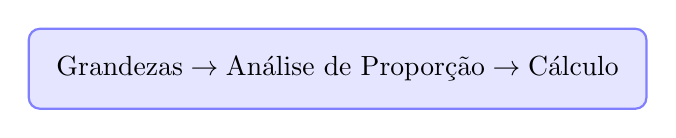
\begin{tikzpicture}
\node[rectangle, fill=blue!10, rounded corners, inner sep=10pt, draw=blue!50, thick] (box) {
$\displaystyle \text{Grandezas} \rightarrow \text{Análise de Proporção} \rightarrow \text{Cálculo}$
};
\end{tikzpicture}

\textbf{Passo a passo:}
\begin{enumerate}
    \item \textbf{Organizar:} Montar uma tabela com todas as grandezas envolvidas.
    \item \textbf{Comparar:} Isolar a grandeza que contém a incógnita ($x$) e compará-la com cada uma das outras, separadamente.
    \item \textbf{Analisar:} Determinar se a relação é \textbf{diretamente proporcional} (seta no mesmo sentido) ou \textbf{inversamente proporcional} (seta invertida).
    \item \textbf{Calcular:} Montar a proporção. A grandeza da incógnita fica isolada, e as demais são multiplicadas conforme a orientação das setas.
\end{enumerate}

\textbf{Na prática:}
\[
\frac{x}{\text{referência}} = \text{produto das razões} 
\begin{cases}
\text{direta: } \frac{\text{novo}}{\text{antigo}} \\
\text{inversa: } \frac{\text{antigo}}{\text{novo}}
\end{cases}
\]

\section*{Exemplo 1: Diretamente Proporcionais}

\textbf{Problema:} Em uma fábrica, 5 máquinas produzem 1200 peças em 4 dias. Quantas peças 8 máquinas produzirão em 6 dias?

\subsection*{Resolução Passo a Passo}

\textbf{1. Montar a tabela:}
\[
\begin{array}{c|c|c}
\text{Máquinas} & \text{Dias} & \text{Peças} \\
\hline
5 & 4 & 1200 \\
8 & 6 & x
\end{array}
\]

\textbf{2. Analisar as proporções (em relação às peças):}
\begin{itemize}
    \item \textbf{Máquinas $\times$ Peças:} Mais máquinas, mais peças. $\Rightarrow$ \textcolor{blue}{Diretamente Proporcional.}
    \item \textbf{Dias $\times$ Peças:} Mais dias, mais peças. $\Rightarrow$ \textcolor{blue}{Diretamente Proporcional.}
\end{itemize}

\textbf{3. Montar a equação:}
\[
\frac{1200}{x} = \frac{5}{8} \times \frac{4}{6}
\]

\textbf{4. Calcular:}
\[
\frac{1200}{x} = \frac{5 \times 4}{8 \times 6} = \frac{20}{48} = \frac{5}{12}
\]
\[
5x = 1200 \times 12 \Rightarrow 5x = 14400 \Rightarrow x = \frac{14400}{5} = 2880
\]

\textbf{Resposta:} Serão produzidas \textbf{2880 peças}.

\section*{Exemplo 2: Inversamente Proporcionais}

\textbf{Problema:} Para alimentar 15 animais por 10 dias, são necessários 300 kg de ração. Quantos dias durará a ração se houver 20 animais?

\subsection*{Resolução Passo a Passo}

\textbf{1. Montar a tabela:}
\[
\begin{array}{c|c|c}
\text{Animais} & \text{Ração (kg)} & \text{Dias} \\
\hline
15 & 300 & 10 \\
20 & 300 & x
\end{array}
\]

\textbf{2. Analisar as proporções (em relação aos dias):}
\begin{itemize}
    \item \textbf{Animais $\times$ Dias:} Mais animais, menos dias (a ração acaba mais rápido). $\Rightarrow$ \textcolor{red}{Inversamente Proporcional.}
    \item \textbf{Ração $\times$ Dias:} A quantidade de ração é constante (300 kg). Como não muda, essa grandeza não interfere na proporção (ou é uma razão de 1/1).
\end{itemize}

\textbf{3. Montar a equação (invertendo a razão dos animais):}
\[
\frac{10}{x} = \frac{20}{15} \quad \text{(A seta invertida inverte a fração)}
\]

\textbf{4. Calcular:}
\[
\frac{10}{x} = \frac{20}{15} \Rightarrow 20x = 150 \Rightarrow x = \frac{150}{20} = 7,5
\]

\textbf{Resposta:} A ração durará \textbf{7,5 dias}.

\section*{Exemplo 3: Misto (Direta e Inversa)}

\textbf{Problema:} 12 operários, trabalhando 8 horas por dia, constroem 240 metros de muro em 15 dias. Quantos operários são necessários para construir 400 metros de muro em 10 dias, trabalhando 6 horas por dia?

\subsection*{Resolução Passo a Passo}

\textbf{1. Montar a tabela:}
\[
\begin{array}{c|c|c|c}
\text{Operários} & \text{Horas/dia} & \text{Dias} & \text{Muro (m)} \\
\hline
12 & 8 & 15 & 240 \\
x & 6 & 10 & 400
\end{array}
\]

\textbf{2. Analisar as proporções (em relação aos operários):}
\begin{itemize}
    \item \textbf{Horas/dia $\times$ Operários:} Menos horas/dia, preciso de \textcolor{red}{mais operários} para terminar no mesmo prazo? Na verdade, comparando: se diminuem as horas, preciso de \textcolor{red}{mais} operários. $\Rightarrow$ \textcolor{red}{Inversamente Proporcional.}
    \item \textbf{Dias $\times$ Operários:} Menos dias, preciso de \textcolor{red}{mais} operários. $\Rightarrow$ \textcolor{red}{Inversamente Proporcional.}
    \item \textbf{Muro $\times$ Operários:} Mais metros de muro, preciso de \textcolor{blue}{mais} operários. $\Rightarrow$ \textcolor{blue}{Diretamente Proporcional.}
\end{itemize}

\textbf{3. Montar a equação:}

\[
\frac{12}{x} = 
{\color{red}\frac{6}{8}} \; \times \;
{\color{red}\frac{10}{15}} \; \times \;
{\color{blue}\frac{240}{400}}
\]
{\footnotesize
\begin{itemize}
    \item[\textcolor{red}{$\blacktriangleright$}] \textcolor{red}{Horas/dia e Dias:} inversas (invertemos a fração)
    \item[\textcolor{blue}{$\blacktriangleright$}] \textcolor{blue}{Metros de muro:} direta (mantemos a fração)
\end{itemize}
}

\textbf{4. Calcular:}
\[
\frac{12}{x} = \frac{6}{8} \times \frac{10}{15} \times \frac{240}{400}
\]

Simplificando:
\[
\frac{6}{8} = \frac{3}{4},\quad 
\frac{10}{15} = \frac{2}{3},\quad 
\frac{240}{400} = \frac{3}{5}
\]

\[
\frac{12}{x} = \frac{3}{4} \times \frac{2}{3} \times \frac{3}{5} = \frac{18}{60} = \frac{3}{10}
\]

\[
3x = 120 \Rightarrow x = 40
\]

\textbf{Resposta:} \textbf{40 operários}
\section*{Exercícios Propostos}

\begin{enumerate}[leftmargin=*]

\item \textbf{(Produção)} Se 4 impressoras iguais produzem 800 panfletos em 2 horas, quantos panfletos 6 impressoras produzirão em 5 horas?

\item \textbf{(Viagem)} Um carro, a uma velocidade média de 80 km/h, percorre um trajeto em 3 horas. Se a velocidade aumentar para 100 km/h, em quanto tempo fará o mesmo percurso?

\item \textbf{(Obra)} 8 pedreiros constroem um muro de 200 m² em 12 dias. Quantos pedreiros seriam necessários para construir 300 m² em 8 dias?

\item \textbf{(Ração)} Em um hotel com 20 hóspedes, há comida suficiente para 15 dias. Se chegarem mais 5 hóspedes, mantendo a mesma quantidade de comida, por quantos dias a comida durará?

\item \textbf{(Complexo)} 15 operários, trabalhando 9 horas por dia, produzem 1200 peças em 20 dias. Quantas horas por dia deverão trabalhar 18 operários para produzir 1800 peças em 15 dias?

\item \textbf{(Torres)} Uma torneira enche um tanque em 6 horas. Duas torneiras iguais a essa enchem o mesmo tanque em quanto tempo?

\item \textbf{(Custo)} Se 5 costureiras fazem 60 uniformes em 4 dias, quantos uniformes 8 costureiras farão em 6 dias?

\item \textbf{(Energia)} Em uma usina, 8 geradores consomem 2000 litros de combustível em 5 horas. Quantos litros 5 geradores consumirão em 8 horas?

\item \textbf{(Digitação)} 3 digitadores digitam 12 páginas em 2 horas. Quantos digitadores são necessários para digitar 30 páginas em 3 horas?

\item \textbf{(Desafio)} Para asfaltar 30 km de uma estrada, 15 trabalhadores levam 18 dias. Após 6 dias de trabalho, 5 trabalhadores adoeceram e não puderam continuar. Considerando que o ritmo de trabalho se manteve, quantos dias a mais serão necessários para concluir a obra?

\end{enumerate}

\section*{Dicas para Resolver}

\begin{itemize}
    \item \textbf{Identifique a incógnita:} Sempre isole a grandeza que você quer descobrir.
    \item \textbf{Use setas:} Desenhe setas para cima (diretamente proporcional) ou para baixo (inversamente) para não se perder.
    \item \textbf{Simplifique:} Antes de multiplicar tudo, simplifique as frações para facilitar o cálculo.
    \item \textbf{Verifique:} No final, veja se a resposta faz sentido (ex: se aumentam os operários, o tempo deveria diminuir).
\end{itemize}

\end{multicols}

\end{document}
